\documentclass[11pt,border=4pt]{standalone}
\usepackage{amsmath,amssymb,bm,mathtools}
\usepackage[fontset=fandol]{ctex}
\usepackage{tikz}
\usetikzlibrary{arrows.meta,calc,patterns,angles,quotes,decorations.markings,decorations.pathmorphing}
\newcommand{\dd}{\mathop{}\!\mathrm d}
\newcommand{\e}{\mathrm e}
\tikzset{axis/.style={->,>=Stealth,line width=.45pt},world/.style={line width=.8pt},flow/.style={->,>=Stealth,line width=.7pt},ray/.style={->,>=Stealth,line width=.7pt},guide/.style={dashed,line width=.35pt},aux/.style={dashed,line width=.35pt},dim/.style={<->,>=Stealth,line width=.35pt},every node/.style={font=\small},force/.style={->,>=Stealth,very thick},gas/.style={fill=blue!7}}
\begin{document}
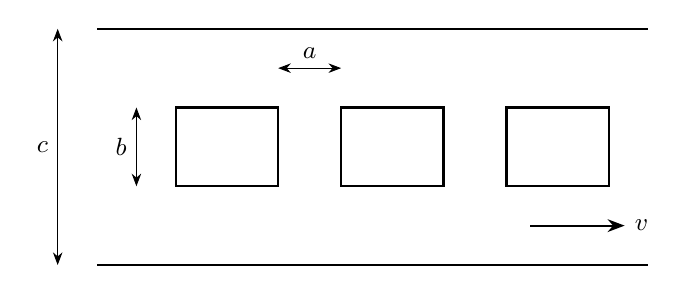
\begin{tikzpicture}\draw[world](-1,0)--(6,0) (-1,3)--(6,3);\foreach \x in {0,2.1,4.2}\draw[world](\x,1)rectangle({\x+1.3},2);\draw[dim](1.3,2.5)--(2.1,2.5)node[midway,above]{$a$};\draw[dim](-.5,1)--(-.5,2)node[midway,left]{$b$};\draw[flow](4.5,.5)--(5.7,.5)node[right]{$v$};\draw[dim](-1.5,0)--(-1.5,3)node[midway,left]{$c$};\end{tikzpicture}
\end{document}
